\documentclass[11pt,a4paper]{article}
\usepackage[hyperref]{acl}
\usepackage{times}
\usepackage{latexsym}
\usepackage{graphicx}
\usepackage{booktabs}
\usepackage{multirow}
\usepackage{amsmath}
\usepackage{xcolor}
\usepackage{soul}

\usepackage[T1]{fontenc}
\usepackage[utf8]{inputenc}
\usepackage{microtype}
\usepackage{inconsolata}

\title{Subword Tokenization Efficiency and Unicode Failure Modes in Bengali Language Modeling}

\author{
  Shifat Islam Santo \\
  The University of Texas at Dallas \\
  \texttt{ShifatIslam.Santo@UTDallas.edu}
}

\begin{document}
\maketitle

\begin{abstract}
We present the first systematic evaluation of subword tokenization strategies for Bengali language modeling, comparing 14 tokenizers across Bengali-dedicated models, multilingual LLMs, and newly trained variants.
On 3,000 held-out Bengali documents, tokenizer choice changes efficiency dramatically: Bengali-dedicated tokenizers achieve 1.47--1.75 tokens per word, while most multilingual alternatives require 7.32--13.69, yielding a 5.0--9.3$\times$ penalty in effective context usage.
We identify a concrete Unicode failure mode behind this gap in our own training runs: omission of a single combining character, U+09BC Bengali Nukta, drives byte-fallback from roughly 2\% to 20\% and accounts for 89.8\% of byte-level tokens in the affected models.
We also document an efficiency--compositionality tradeoff: tokenizers that memorize whole Bengali words maximize fertility, while more decompositional tokenizers may preserve morpheme structure that could help generative generalization.
We release an evaluation framework, 13 trained tokenizers, and a benchmark construction recipe to support future Bengali NLP research.
\end{abstract}

\section{Introduction}

Bengali (Bangla) is the seventh most spoken language globally with over 230 million native speakers, yet it remains underrepresented in the current landscape of large language models.
Recent work has begun to address this gap: LilTii \cite{liltii2026}, a 670M-parameter model trained from scratch, demonstrated that a well-designed Bengali tokenizer was a key factor in achieving competitive performance with substantially less compute than Qwen3-0.6B.

Despite this, no systematic study exists comparing tokenization strategies for Bengali.
Practitioners building Bengali language models face an uninformed choice between (a) repurposing multilingual tokenizers from models like Llama or Qwen, (b) adopting tokenizers from Bengali encoder models like BanglaBERT \cite{banglabert2022}, or (c) training new tokenizers from scratch.
Each choice carries implications for training efficiency and inference cost, yet these tradeoffs have not been quantified.

In this work, we evaluate 14 tokenizers spanning four categories: Bengali-dedicated encoder tokenizers, Bengali LLM tokenizers, newly trained tokenizers with varied configurations, and multilingual LLM tokenizers.
We evaluate along five dimensions: fertility (tokens per word), compression ratio (bytes per token), byte-fallback rate, morphological segmentation quality, and effective context capacity.

Our key contributions are:
\begin{enumerate}
    \item The first systematic comparison of tokenizer strategies for Bengali, covering 14 tokenizers across 4 categories.
    \item Quantification of a large \textbf{Bengali tokenization efficiency gap}: most widely used multilingual tokenizers are 5--9$\times$ less efficient for Bengali than dedicated alternatives, though not all multilingual tokenizers are equally poor (BLOOM at 1.75 is competitive).
    \item Quantitative evidence that a \textbf{single missing combining character} (U+09BC Bengali Nukta) accounts for 89.8\% of byte-fallback tokens in affected tokenizers, driving a rate increase from 2\% to 20\%.
    \item Preliminary analysis of an \textbf{efficiency--compositionality tradeoff}: tokenizers that memorize whole Bengali words achieve superior fertility but sacrifice morphological decomposition that may benefit generative model generalization.
\end{enumerate}

\section{Background}

\subsection{Bengali Script Characteristics}

Bengali (Eastern Nagari) is an abugida script occupying the Unicode range U+0980--U+09FF with 96 assigned code points.
The script presents several challenges for subword tokenization:

\textbf{Conjunct consonants.} Bengali forms conjuncts (yuktakshar) by combining consonants with the hasanta (virama, U+09CD). The word \textit{bisshobidyaloy} (university) contains three conjuncts, producing a visually compact but computationally complex string.

\textbf{Combining marks.} Characters like the Nukta (U+09BC) modify base characters to represent sounds from other languages. These combining marks are essential for correct representation but are easily lost during normalization.

\textbf{Morphological richness.} Bengali is an agglutinative language with productive case marking, postpositions, and derivational morphology. A single root can generate dozens of surface forms (e.g., \textit{sarkar} $\rightarrow$ \textit{sarkari} $\rightarrow$ \textit{sarkaribhabe}).

\subsection{Subword Tokenization}

Modern language models use subword tokenization to balance vocabulary size against coverage.
Byte Pair Encoding (BPE) \cite{sennrich2016bpe} greedily merges the most frequent character pairs; Unigram \cite{kudo2018unigram} optimizes a probabilistic model over a large initial vocabulary.
Both approaches depend heavily on training data quality and composition.

\subsection{Related Work}

\textbf{Multilingual tokenization.} \citet{ahia2023do} showed that tokenizer fertility varies 15$\times$ across languages for the same model, directly impacting the cost of processing non-English text.
\citet{petrov2024language} introduced fertility as a key metric for comparing tokenization efficiency across languages.

\textbf{Bengali NLP.} BanglaBERT \cite{banglabert2022} trained a 32K ELECTRA-style tokenizer on 27.5GB of Bengali text, achieving state-of-the-art results on Bengali NLU benchmarks.
BanglaT5 \cite{banglat5} extended this to sequence-to-sequence tasks.
LilTii \cite{liltii2026} trained a 49K BPE tokenizer on Bengali+English data, reporting a fertility of 1.66 tokens per word.
TituLLM \cite{titulm2025} and TigerLLM \cite{tigerllm2025} used extended Llama tokenizers for Bengali continued pretraining.

No prior work has systematically compared these tokenization approaches on controlled benchmarks.

\section{Methodology}

\subsection{Evaluation Data}

We construct a held-out evaluation set of 3,000 Bengali documents sampled from the last 10,000 entries of a 1.2M-document Bengali web corpus, ensuring no overlap with the training split used for our newly trained tokenizers and Kotha-1.
Documents are filtered to a minimum length of 200 characters.
The corpus comprises cleaned and deduplicated text from CulturaX \cite{culturax2024}, Bengali Wikipedia, and Sangraha \cite{sangraha2024}, processed through NFKC normalization and Bengali-specific cleaning.

\subsection{Tokenizers Evaluated}

We evaluate 14 tokenizers across four categories:

\textbf{Bengali encoder tokenizers} (2): BanglaBERT and BanglaT5 \cite{banglabert2022,banglat5}, both 32K vocabularies trained on the Bangla2B+ corpus. These two models share the same tokenizer, which accounts for their identical metrics in Table~\ref{tab:main}.

\textbf{Bengali LLM tokenizers} (2): Kotha-1 (our prior work; 32K BPE trained on 1.5GB Bengali text with NFC normalization) and LilTii v0.2 \cite{liltii2026} (49K BPE trained on Bengali+English).

\textbf{Newly trained tokenizers} (5): We train tokenizers across two axes---algorithm (BPE vs.\ Unigram) and vocabulary size (32K, 49K, 64K)---on 1.5GB sampled from the Bengali corpus using SentencePiece \cite{kudo2018sentencepiece} with byte-fallback enabled, identity normalization, character coverage 0.9999, and seed 42. As discussed in Section~\ref{sec:nukta}, these tokenizers suffer from a normalization artifact that elevates byte-fallback rates; conclusions drawn from their relative comparisons should be interpreted cautiously.

\textbf{Multilingual LLM tokenizers} (5): Qwen-2.5 (152K vocab), BLOOM-560m (251K), TinyLlama (32K, Llama-2 family), Phi-2 (50K), and StableLM-2 (100K).

\subsection{Metrics}

\textbf{Fertility.} Average number of tokens per whitespace-delimited word, following \citet{ahia2023do}. Lower is better.

\textbf{Compression ratio.} Average bytes of UTF-8 text per token. Higher indicates more efficient encoding.

\textbf{Byte-fallback rate.} Percentage of output tokens that are byte-level fallback tokens (\texttt{<0xAB>}), indicating characters the tokenizer failed to learn.

\textbf{Morphological probe score.} Average tokens per word on a curated set of 20 morphologically diverse Bengali words covering compounds (e.g., \textit{bisshobidyaloy}), case-marked forms (\textit{bangladesher}), loanwords (\textit{computer}), and derivations (\textit{sarkaribhabe}).

\textbf{Effective context capacity.} Kilobytes of Bengali text encodable in a fixed 4,096-token window, computed as $4096 \times \text{bytes/token} / 1024$.

\section{Results}

\subsection{The Bengali Tokenization Efficiency Gap}

Table~\ref{tab:main} presents the complete evaluation results, with fertility visualized in Figure~\ref{fig:fertility}.

\begin{figure}[t]
\centering
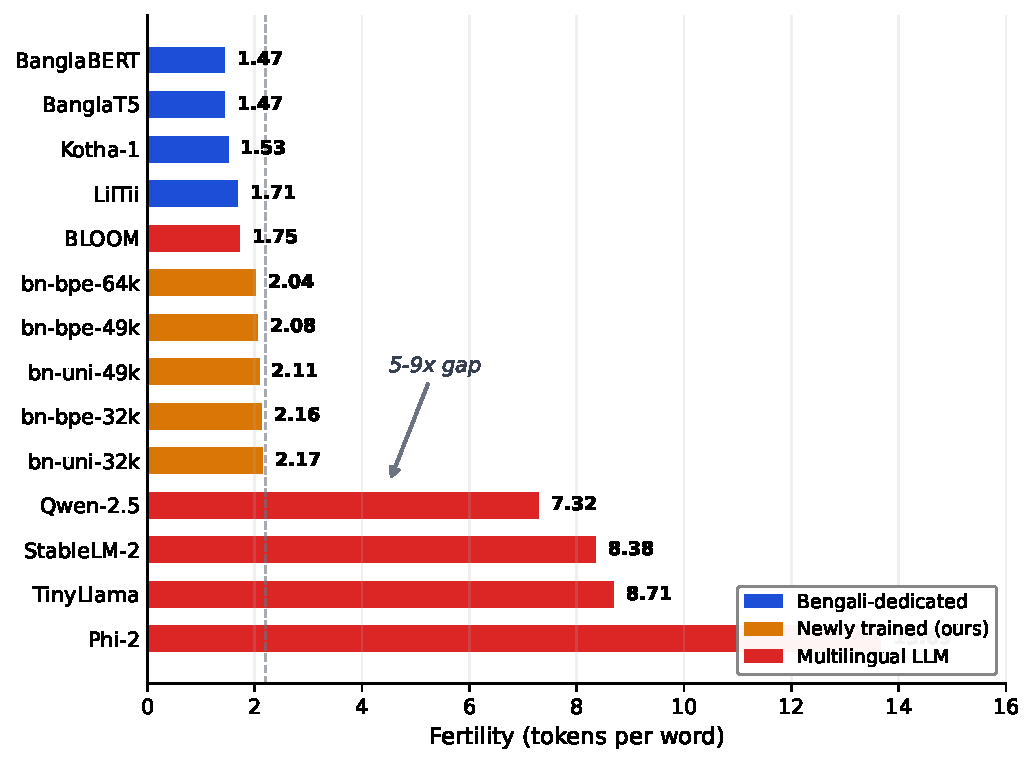
\includegraphics[width=\columnwidth]{figures/fertility_comparison.pdf}
\caption{Fertility (tokens per word) across tokenizers on Bengali text. Bengali-dedicated tokenizers cluster below 2.0; most multilingual LLM tokenizers range from 7.3 to 13.7. BLOOM is the exception among multilingual models.}
\label{fig:fertility}
\end{figure}

\begin{table*}[!ht]
\centering
\small
\begin{tabular}{llrrrrrr}
\toprule
\textbf{Tokenizer} & \textbf{Category} & \textbf{Vocab} & \textbf{Fertility}$\downarrow$ & \textbf{B/Tok}$\uparrow$ & \textbf{ByteFB\%}$\downarrow$ & \textbf{Probes}$\downarrow$ & \textbf{KB/4K}$\uparrow$ \\
\midrule
BanglaBERT & Bengali Enc. & 32K & \textbf{1.47} & \textbf{12.42} & 0.0 & \textbf{1.1} & \textbf{49.7} \\
BanglaT5 & Bengali Enc. & 32K & \textbf{1.47} & \textbf{12.42} & 0.0 & \textbf{1.1} & \textbf{49.7} \\
Kotha-1 & Bengali LLM & 32K & 1.53 & 11.95 & 1.9 & \textbf{1.1} & 47.8 \\
LilTii v0.2 & Bengali LLM & 49K & 1.71 & 10.68 & 1.6 & 2.6 & 42.7 \\
BLOOM & Multilingual & 251K & 1.75 & 10.47 & 0.0 & 2.2 & 41.9 \\
\midrule
bn-bpe-64k & New (ours)$^\dagger$ & 64K & 2.04 & 8.96 & 21.2 & 1.7 & 35.8 \\
bn-bpe-49k & New (ours)$^\dagger$ & 49K & 2.08 & 8.81 & 20.9 & 1.7 & 35.2 \\
bn-uni-49k & New (ours)$^\dagger$ & 49K & 2.11 & 8.67 & 20.5 & 1.7 & 34.7 \\
bn-bpe-32k & New (ours)$^\dagger$ & 32K & 2.16 & 8.48 & 20.1 & 1.7 & 33.9 \\
bn-uni-32k & New (ours)$^\dagger$ & 32K & 2.17 & 8.42 & 19.9 & 2.0 & 33.7 \\
\midrule
Qwen-2.5 & Multilingual & 152K & 7.32 & 2.50 & 0.0 & 10.7 & 10.0 \\
StableLM-2 & Multilingual & 100K & 8.38 & 2.18 & 0.0 & 13.4 & 8.7 \\
TinyLlama & Multilingual & 32K & 8.71 & 2.10 & 0.0 & 12.8 & 8.4 \\
Phi-2 & Multilingual & 50K & 13.69 & 1.34 & 0.0 & 21.9 & 5.4 \\
\bottomrule
\end{tabular}
\caption{Tokenizer evaluation on 3,000 Bengali documents. Fertility = tokens per word. B/Tok = bytes per token. ByteFB\% = byte-fallback token percentage. Probes = average tokens on 20 morphological probe words. KB/4K = kilobytes of Bengali text in a 4,096-token context window ($4096 \times \text{B/Tok} / 1024$). $^\dagger$These tokenizers are affected by the normalization artifact described in Section~\ref{sec:nukta}.}
\label{tab:main}
\end{table*}

Bengali-dedicated tokenizers achieve fertility between 1.47 and 1.75 tokens per word.
Most multilingual LLM tokenizers range from 7.32 (Qwen-2.5) to 13.69 (Phi-2)---a \textbf{5.0--9.3$\times$} difference.
Notably, BLOOM (1.75) is the exception: despite being multilingual, its 251K vocabulary includes substantial Bengali coverage, placing it in the same range as dedicated Bengali tokenizers.
This suggests that the efficiency gap is driven by tokenizer design and script coverage rather than being an inherent property of multilingual models.

In terms of effective context capacity, at 4,096 tokens BanglaBERT's tokenizer encodes 49.7~KB of Bengali text, while Phi-2 encodes only 5.4~KB---a 9.2$\times$ difference.
Equivalently, using fertility: BanglaBERT fits $4096/1.47 \approx 2{,}786$ Bengali words in a 4,096-token window, while Phi-2 fits only $4096/13.69 \approx 299$ words.

\subsection{Observations on Vocabulary Size}

Among the well-trained tokenizers in our evaluation (BanglaBERT at 32K, Kotha-1 at 32K, LilTii at 49K), we do not observe a clear intrinsic advantage for larger vocabularies in this range: BanglaBERT achieves 1.47 fertility at 32K while LilTii achieves 1.71 at 49K. However, these models differ in training data and recipe, so this is a cross-model observation rather than a controlled comparison of vocabulary size.

Among our newly trained tokenizers, increasing vocabulary from 32K to 64K improves fertility by only 5.5\% (2.16 $\rightarrow$ 2.04 for BPE).
However, because these tokenizers are affected by the normalization artifact described in Section~\ref{sec:nukta}, this comparison should be interpreted with caution.

\subsection{BPE and Unigram Under Our Setup}

At matched vocabulary sizes within our newly trained tokenizers, BPE and Unigram show minimal differences: at 32K, BPE achieves 2.16 fertility versus Unigram's 2.17; at 49K, 2.08 versus 2.11.
This contrasts with findings for morphologically rich languages like Turkish where Unigram shows clearer advantages \cite{toraman2023impact}.
We note that this comparison is confounded by the shared normalization artifact, and we do not claim this generalizes beyond our specific setup.

\section{Analysis}

\subsection{The Nukta Problem: Training Data Sensitivity}
\label{sec:nukta}

Our most surprising finding concerns the byte-fallback rates of our newly trained tokenizers.
Despite training on 1.5GB of Bengali text from the same corpus used for Kotha-1, our new tokenizers exhibit $\sim$20\% byte-fallback rates compared to 1.9\% for Kotha-1.

We traced this to the Bengali Nukta character (U+09BC), a combining mark that modifies base consonants.
Table~\ref{tab:nukta} summarizes our forensic analysis.
Vocabulary inspection confirms that U+09BC is present as a learned token in the Kotha-1 vocabulary but absent from our newly trained tokenizers, where it decomposes into three byte-level tokens (0xE0, 0xA6, 0xBC) at each occurrence.

\begin{table}[h]
\centering
\small
\setlength{\tabcolsep}{4pt}
\begin{tabular}{@{}lcc@{}}
\toprule
& \textbf{Kotha-1} & \textbf{New} \\
\midrule
Bengali chars as single tok & 74 & 71 \\
Bengali chars as byte-fallback & 22 & 25 \\
U+09BC in vocabulary & Yes & No \\
Mismatched characters & \multicolumn{2}{c}{3 (incl.\ U+09BC)} \\
Document-level byte-FB\% & 1.9\% & 20.0\% \\
\midrule
\multicolumn{3}{@{}l@{}}{\textit{U+09BC attribution (on 2K eval docs):}} \\
U+09BC occurrences in text & \multicolumn{2}{c}{167,207 (1.88\% of chars)} \\
Byte-FB tokens from U+09BC & \multicolumn{2}{c}{501,621 (3 per occurrence)} \\
Share of all byte-FB tokens & \multicolumn{2}{c}{89.8\%} \\
Byte-FB\% excluding U+09BC & \multicolumn{2}{c}{2.03\%} \\
\bottomrule
\end{tabular}
\caption{Forensic analysis of byte-fallback between Kotha-1 and newly trained tokenizers. U+09BC (Nukta) is absent from the new tokenizer vocabulary and accounts for 89.8\% of all byte-fallback tokens. Excluding U+09BC, the byte-fallback rate drops to 2.03\%, matching Kotha-1.}
\label{tab:nukta}
\end{table}

Quantitative analysis confirms U+09BC as the dominant factor: removing its contribution reduces the byte-fallback rate from 20.0\% to 2.03\%, closely matching Kotha-1's 1.9\%.
The other two mismatched characters (U+09F0, U+09F7) appear fewer than 30 times each in the evaluation data and contribute negligibly.

The root cause is a normalization difference: Kotha-1 was trained on NFC-normalized text where the Nukta appears composed with base characters, while our new training sample contained a higher proportion of NFD-decomposed sequences.
We have not yet retrained with corrected normalization to confirm this directly, though the quantitative attribution is strong.

This finding suggests that \textbf{languages using combining marks are sensitive to normalization choices in tokenizer training data}, and that practitioners should verify combining character coverage after training.

\subsection{Efficiency vs.\ Compositionality}

Table~\ref{tab:probes} illustrates a tension between tokenization efficiency and morphological decomposition.

\begin{table}[h]
\centering
\small
\setlength{\tabcolsep}{3pt}
\begin{tabular}{@{}lll@{}}
\toprule
\textbf{Word (romanized)} & \textbf{BERT} & \textbf{LilTii} \\
\midrule
\textit{bangladesh} & 1 tok & 1 tok \\
\textit{bangladesher} (gen.) & 1 tok & bangla+desher \\
\textit{bisshobidyaloy} (univ.) & 1 tok & 3 tok \\
\textit{bisshobidyaloygulote} & 2 tok & 4 tok \\
\textit{antorjatik} (intl.) & 1 tok & 3 tok \\
\textit{computer} (loan) & 1 tok & 3 tok \\
\textit{sarkaribhabe} (adv.) & 1 tok & sarkari+bhabe \\
\bottomrule
\end{tabular}
\caption{Morphological segmentation examples from a 20-word probe set spanning compounds, case-marked forms, loanwords, and derivations. BanglaBERT memorizes whole words; LilTii decomposes at morpheme boundaries. Parenthetical annotations indicate word type.}
\label{tab:probes}
\end{table}

BanglaBERT and Kotha-1 memorize common Bengali words as single tokens, producing excellent fertility (1.47) but treating ``\textit{bangladesh}'' and ``\textit{bangladesher}'' as unrelated vocabulary items.
LilTii decomposes morphologically: ``\textit{bangladesher}'' becomes ``bangla'' + ``desher'', and ``\textit{sarkaribhabe}'' becomes ``sarkari'' + ``bhabe''.
This sacrifices fertility (1.71) but potentially enables the model to learn that the genitive suffix ``-er'' generalizes across nouns.

This tradeoff parallels findings in morphologically rich languages like Finnish and Turkish \cite{virpioja2013morphological}, but has not been previously documented for Bengali.
We note that our probe set of 20 words is illustrative rather than exhaustive; a larger-scale morphological evaluation is needed to draw firm conclusions about downstream impact.

\subsection{Context Window Implications}

The practical impact of tokenizer choice is most visible through effective context capacity.
In a 4,096-token context window:

\begin{itemize}
    \item BanglaBERT: 49.7 KB ($\approx$2,800 words)
    \item LilTii: 42.7 KB ($\approx$2,400 words)
    \item Qwen-2.5: 10.0 KB ($\approx$560 words)
    \item Phi-2: 5.4 KB ($\approx$300 words)
\end{itemize}

\noindent where word counts are derived as $4096 / \text{fertility}$.
A model using Phi-2's tokenizer would need a $\sim$37,000-token context window to match the Bengali word coverage of a 4,096-token model using BanglaBERT's tokenizer.
This is consistent with the hypothesis that the tokenizer bottleneck may limit the effectiveness of continuing pretraining multilingual LLMs on Bengali data, though we have not tested downstream performance directly.

\section{Discussion}

\textbf{Recommendations for practitioners.} Based on our intrinsic evaluation, we suggest:
(1) Prefer a tokenizer with demonstrated Bengali coverage rather than defaulting to the tokenizer inherited from a multilingual base model---though as BLOOM shows, some multilingual tokenizers can achieve competitive Bengali efficiency.
(2) Ensure training data undergoes consistent NFC Unicode normalization before tokenizer training, with explicit verification that combining marks (especially U+09BC Nukta) are represented as learned tokens.
(3) Consider the efficiency--compositionality tradeoff based on the target task.

\textbf{Implications for continued pretraining.} Our results are consistent with the hypothesis that continuing pretraining Llama or Qwen on Bengali data \cite{titulm2025,tigerllm2025} faces a tokenizer efficiency bottleneck, since those tokenizers process 5--9$\times$ fewer Bengali words per context window.
This may partly explain why from-scratch models like LilTii achieve competitive results, though other factors (architecture, data quality) likely contribute.

\textbf{Generalization.} The Nukta sensitivity finding likely generalizes to other Indic scripts (Devanagari, Gurmukhi, Gujarati) and any writing system using combining marks.
We encourage researchers to audit tokenizer training data for normalization consistency.

\textbf{Limitations.} Our evaluation uses a single Bengali web corpus, which may not represent all text domains.
We do not evaluate downstream language modeling performance; all conclusions are based on intrinsic tokenization metrics.
Our newly trained tokenizers are affected by a normalization artifact (Section~\ref{sec:nukta}), which confounds comparisons of vocabulary size and algorithm choice within that group.
The morphological probe analysis uses only 20 hand-selected words and is illustrative rather than systematic.
The Nukta diagnosis, while well-supported by vocabulary inspection, has not been confirmed via ablation (retraining with corrected normalization).

\section{Conclusion}

We presented a systematic evaluation of subword tokenization for Bengali, comparing 14 tokenizers across four categories.
Our results reveal that most popular multilingual LLM tokenizers are 5--9$\times$ less efficient for Bengali than dedicated alternatives, with BLOOM being a notable exception.
In a 4,096-token context window, this translates to an effective capacity difference of 49.7~KB vs.\ 5.4~KB of Bengali text.
We identified an acute sensitivity to Unicode normalization in tokenizer training: the absence of a single combining character (U+09BC) accounts for 89.8\% of byte-fallback tokens in affected tokenizers, driving rates from 2\% to 20\%.
We documented a preliminary efficiency--compositionality tradeoff and provided practical recommendations for Bengali tokenizer design.

We release our evaluation framework, trained tokenizers, and benchmark data at \url{https://github.com/oneKn8/bengali-tokenizer-eval}.

\bibliography{references}

\end{document}
